\documentclass[11pt]{book}

%\usepackage[width=7.0in, height=9.0in, top=1.0in, papersize={8.5in,11in}]{geometry}
%\usepackage[pdftex]{graphicx}
%\usepackage{datetime}
%\usepackage{anyfontsize}
%\usepackage{t1enc}
%\usepackage{verbatim}
%\usepackage{algorithm}
%\usepackage{algorithmic}
%\usepackage{framed}
%\usepackage{pdfpages}
%\usepackage[export]{adjustbox}
%\usepackage{listings}
%\lstset{language=C}

\lstset{language=python,frame=ltrb,framesep=5pt,basicstyle=\normalsize,
 keywordstyle=\ttfamily\color{DarkRed},
%morecomment=[n][\textbf]{In\ [}{]\:},
%morecomment=[n][\textbf]{Out\ [}{]\:},
morecomment=[s][\color{blue}]{In\ [}{]\:},
morecomment=[s][\color{red}]{Out[}{]\:},
identifierstyle=\ttfamily\color{DarkBlue}\bfseries,
commentstyle=\color{DarkGreen},
stringstyle=\ttfamily,
showstringspaces=false,tabsize = 3}


\lstdefinelanguage{shell} {
commentstyle = \color{black},
keywordstyle = \color{black},
stringstyle = \color{black},
identifierstyle = \color{black},
morecomment=[s][\color{blue}]{In\ [}{]\:},
morecomment=[s][\color{red}]{Out[}{]\:},
 }

\pagestyle{empty}

%\usepackage{helvet}
\renewcommand{\familydefault}{\sfdefault}

\begin{document}

%{\fontsize{16}{16}\selectfont Sprint Report \#5}

\section*{Team Overview}
\hrulefill
\subsection*{Members}
Mackenzie Smith, Alex Nienhueser

\subsection*{Project Title}
Dahl Virtual Museum Tour

\subsection*{Company}
Dahl Arts Center


\section*{Sprint Report}

\hrulefill
\subsection*{Work Accomplished}
\begin{itemize}
\item Created rough alternate environment
\item Added in all remaining paintings and text descriptions


\end{itemize}
\subsection*{Work Left}
\begin{itemize}
\item User documentation
\item Fix issue of video and sound synchronization
\item Finalize the menu system
\end{itemize}

\section*{Sprint Overview}
The main feature added during this sprint was the alternate environment.  During our initial meeting with the Dahl Arts Center, when the design team brought up the idea of an alternate environment, the Arts Center thought of using the Black Hills as the chosen environment.  This environment would basically be another room to view the paintings in, except this one will be outdoors on a plateau.  The paintings will be in the same order but the walls will be replaced with wooden fences to allow the user to see outside into the hills.


Originally this sounded like a challenge because of the lack of 3D model design skill in our team, however after some research into the Unreal Engine height map support, we found we could import a height map directly into the engine.  This allowed the design team to use Google Maps to generate a height map of a portion of the Black Hills and use it as a landscape.  Textures and other objects to make it more realistic need to be applied, such as grass, trees, and a sky. 
 
\section*{Alternate Environment}
The design process for the alternate environments wasn't that involved.  After the Dahl Arts Center decided on the Black Hills as the other environment, the design team went about thinking of different ways it could be done.  One method was very crude and that was to go out into the hills and take a panoramic photo of the horizon and use that as a texture for an in-engine object. This would have captured the realistic flora of the Black Hills, but would also be very limited to the camera resolution which might end up looking pixelated.  

The method the design team decided on was to use the height maps generated from Google Maps. A section of the Black Hills was selected, with no real selection process, and then imported into the Unreal Engine with its built in height map extension.  This way, the actual Black Hills will be represented in the engine, however there will be some downfalls mainly with authenticity. 

To make the virtual reality Black Hills appear as authentic as possible, trees and grass and other shrubs will be placed around the environment to give the appearance of the flora of the Black Hills.  This is not the case however since the objects in the engine are not actual representations of the actual plants in the Black Hills, such as the Black Hills Spruce or Ponderosa Pine.

\section*{Client Interactions}
Dr. Adkins as well as the design team were very busy during this sprint, this resulted in very limited client interactions.  Emails were sent back and forth to maintain communication, and there will be a meeting on Monday the 21st to show how the project is coming so far. 
	
\section*{Screenshots}
\begin{figure}
\caption{The gallery was copied from the room and moved into the open space}
\centering
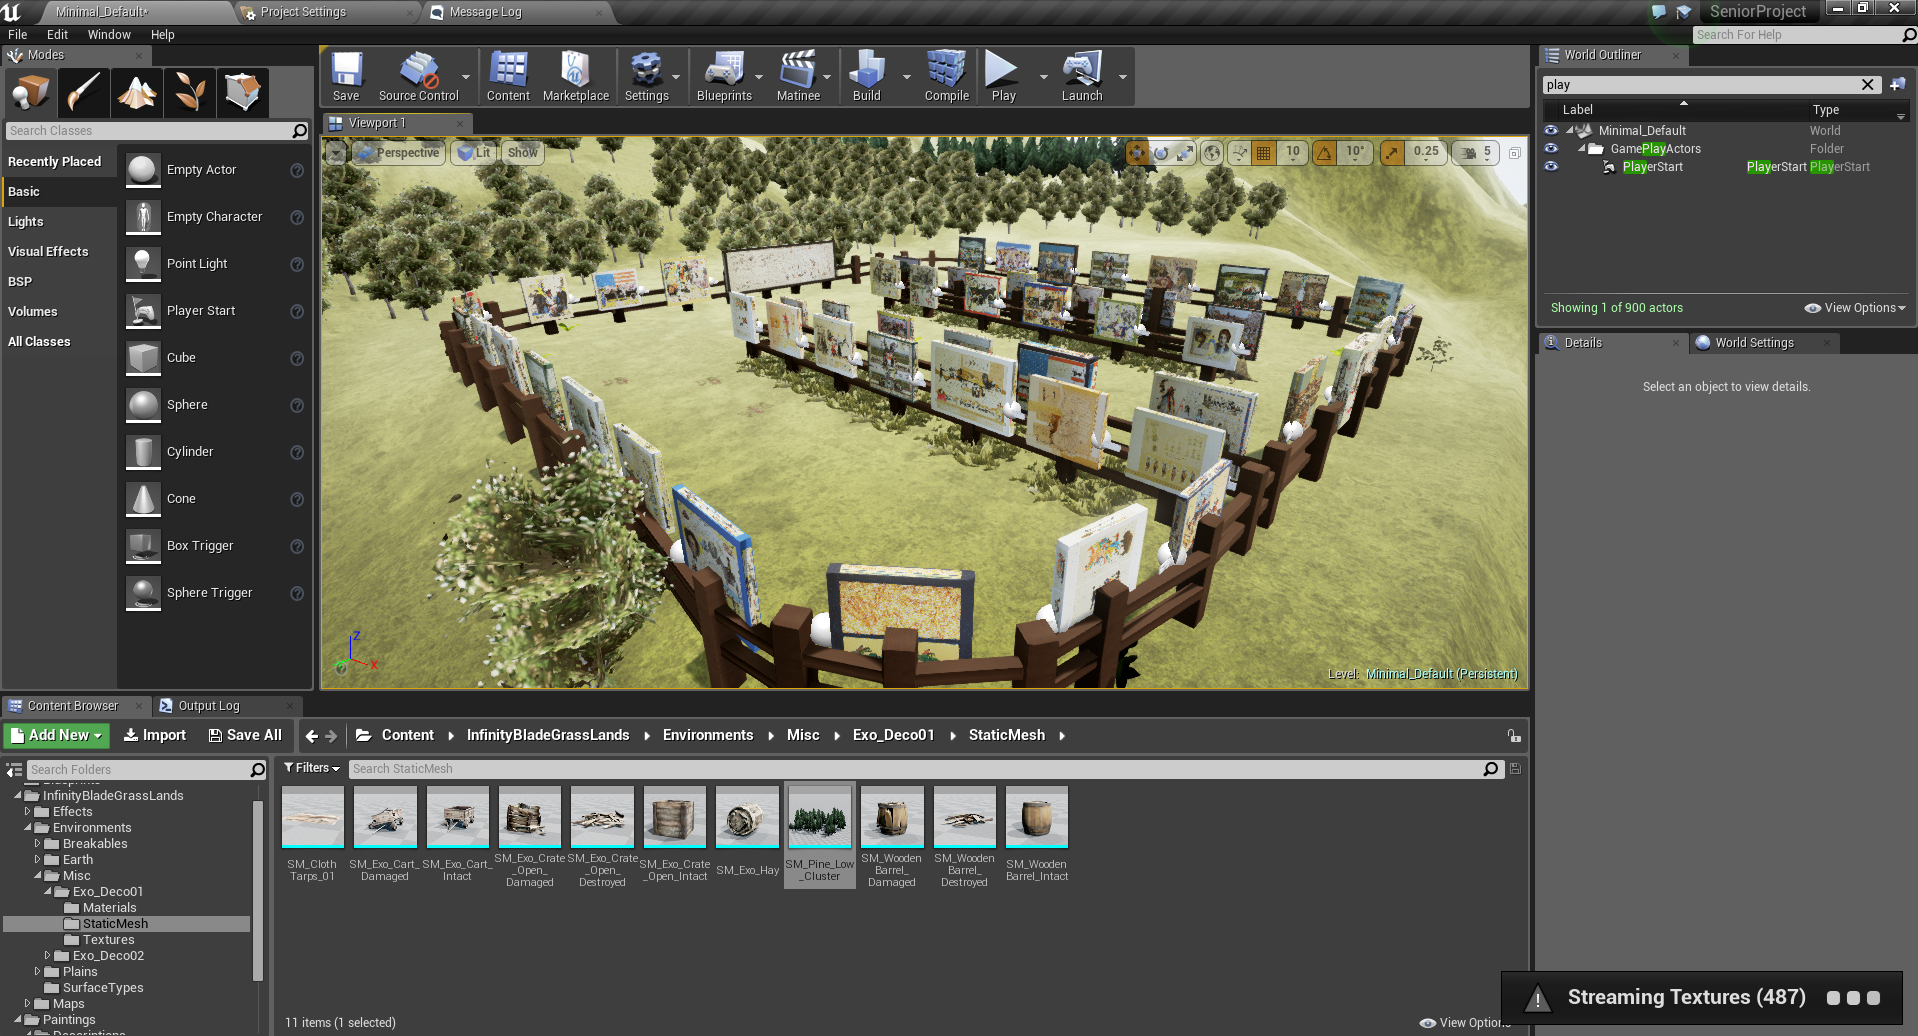
\includegraphics[scale=0.40]{Pic1.png}
\end{figure}

\begin{figure}
\caption{As you can see, the fences replaced the walls for the paintings to hang on}
\centering
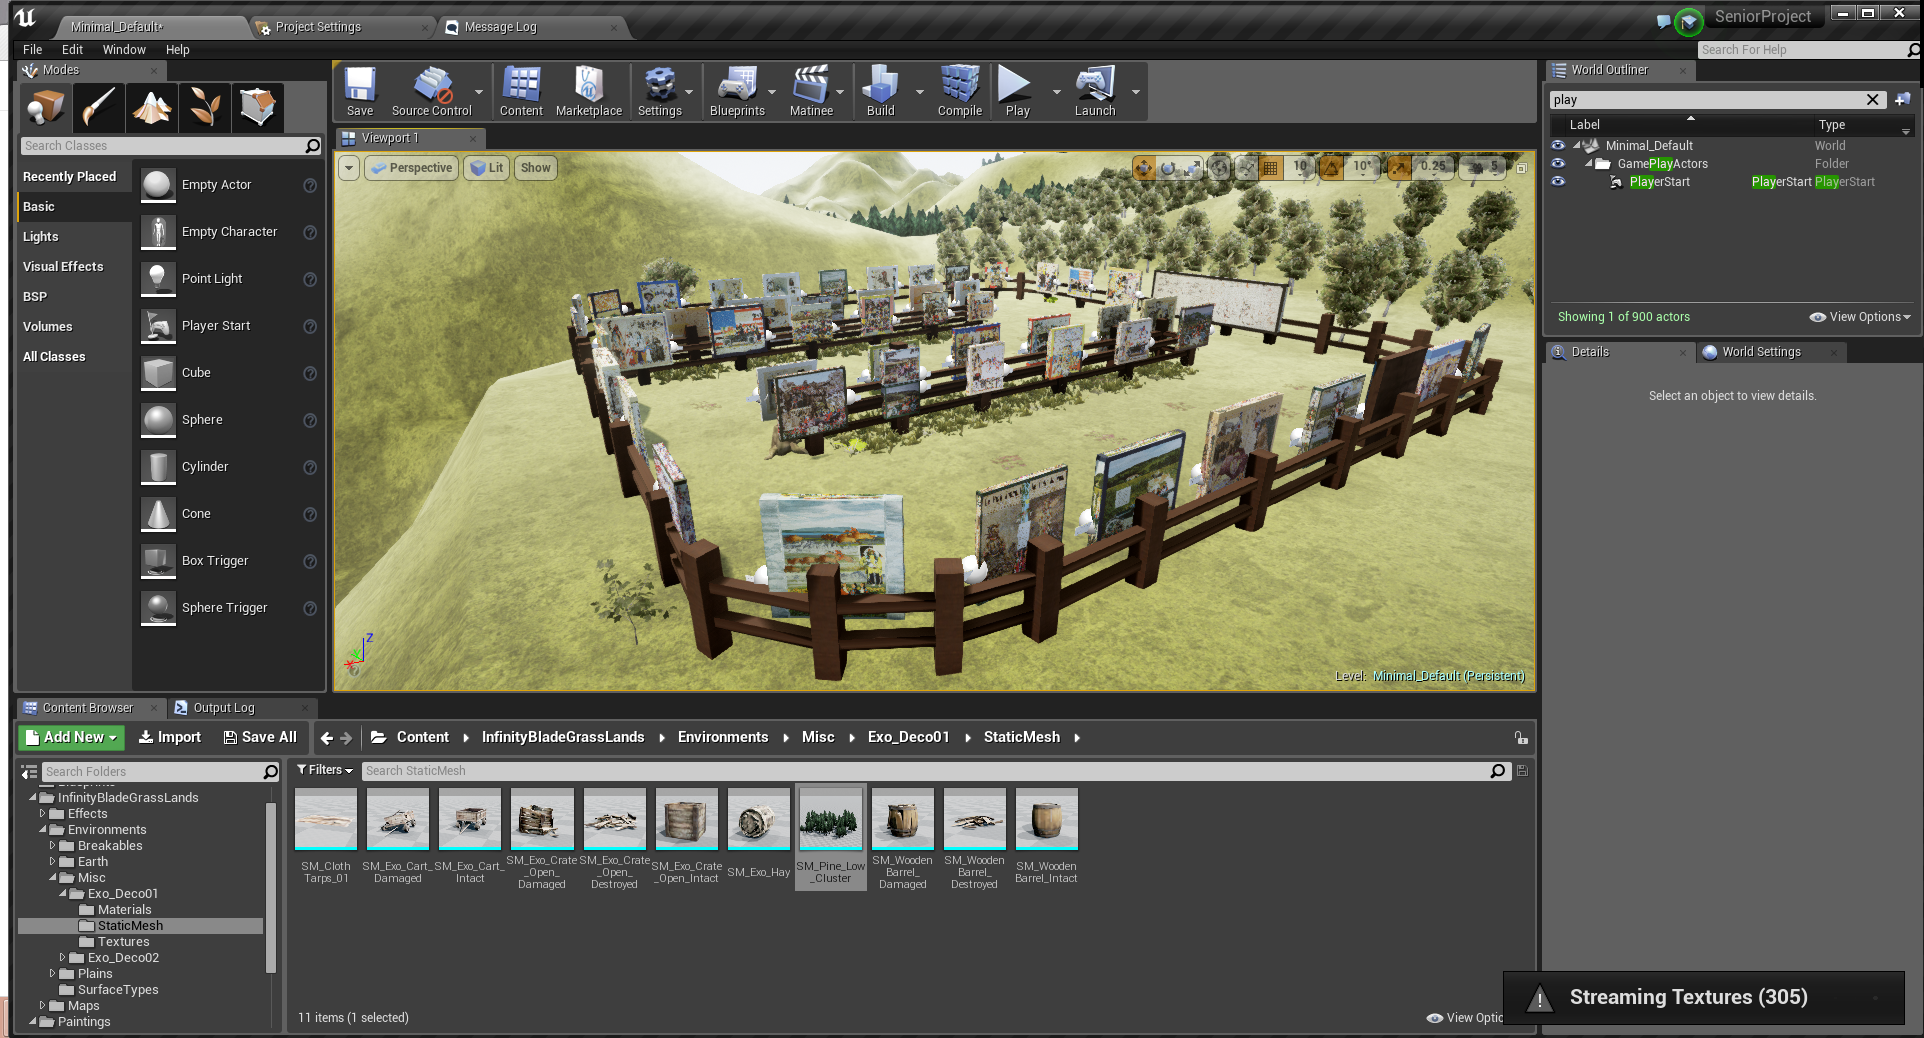
\includegraphics[scale=0.40]{Pic2.png}
\end{figure}

\section*{Issues}
\begin{itemize}
\item Like mentioned above, the authenticity of the plants in the environment is lacking
\end{itemize}

\end{document}
